%%%%%%%%%%%%%%%%%%%%%%%%%%%%%%%%%%%%%%%%%%%%%%%%%%%%%%%%%%%%%%%%%%%%%
%% This is a (brief) model paper using the achemso class
%% The document class accepts keyval options, which should include
%% the target journal and optionally the macuscript tye
%%%%%%%%%%%%%%%%%%%%%%%%%%%%%%%%%%%%%%%%%%%%%%%%%%%%%%%%%%%%%%%%%%%%%
\documentclass[journal=jacsat,manuscript=article]{achemso}

%%%%%%%%%%%%%%%%%%%%%%%%%%%%%%%%%%%%%%%%%%%%%%%%%%%%%%%%%%%%%%%%%%%%%
%% Place any additional packages needed here.  Only include packages
%% which are essential, to avoid problems later.
%%%%%%%%%%%%%%%%%%%%%%%%%%%%%%%%%%%%%%%%%%%%%%%%%%%%%%%%%%%%%%%%%%%%%
\usepackage[version=3]{mhchem} % Formula subscripts using \ce{}
\usepackage{graphicx}

%%%%%%%%%%%%%%%%%%%%%%%%%%%%%%%%%%%%%%%%%%%%%%%%%%%%%%%%%%%%%%%%%%%%%
%% If issues arise when submitting your manuscript, you may want to
%% un-comment the next line.  This provides information on the
%% version of every file you have used.
%%%%%%%%%%%%%%%%%%%%%%%%%%%%%%%%%%%%%%%%%%%%%%%%%%%%%%%%%%%%%%%%%%%%%
%%\listfiles

%%%%%%%%%%%%%%%%%%%%%%%%%%%%%%%%%%%%%%%%%%%%%%%%%%%%%%%%%%%%%%%%%%%%%
%% Place any additional macros here.  Please use \newcommand* where
%% possible, and avoid layout changing macros (which are not used
%% when typesetting).
%%%%%%%%%%%%%%%%%%%%%%%%%%%%%%%%%%%%%%%%%%%%%%%%%%%%%%%%%%%%%%%%%%%%%
\newcommand*{\mycommand}[1]{\texttt{\emph{#1}}}

%%%%%%%%%%%%%%%%%%%%%%%%%%%%%%%%%%%%%%%%%%%%%%%%%%%%%%%%%%%%%%%%%%%%%
%% Meta-data block
%% ---------------
%% Each author should be given as a separate \author command.
%%
%% Corresponding authors should have an e-mail given after the author
%% name as an \email command.
%%
%% The affiliation of authors is given after the authors; each
%% \affiliation command applies to all preceding authors not already
%% assigned an affiliation.
%%
%% The affiliation takes an option argument for the short name.  This
%% will typically be something like "University of Somewhere".
%%
%% The \altaffiliation macro should be used for new address, etc.
%%%%%%%%%%%%%%%%%%%%%%%%%%%%%%%%%%%%%%%%%%%%%%%%%%%%%%%%%%%%%%%%%%%%%
\author{Robert Jensen}
\author{Thomas Andersen}
\author{Anders Nierhoff}
\author{Thomas Pedersen}
\author{Ole Hansen}
\author{S\o ren Dahl}
\author{Ib Chorkendorff}
\email{ibchork@fysik.dtu.dk}

%%%%%%%%%%%%%%%%%%%%%%%%%%%%%%%%%%%%%%%%%%%%%%%%%%%%%%%%%%%%%%%%%%%%%
%% The document title should be given as usual
%% A short title can be given as a *suggestion* for running headers.
%%%%%%%%%%%%%%%%%%%%%%%%%%%%%%%%%%%%%%%%%%%%%%%%%%%%%%%%%%%%%%%%%%%%%
\title[Oxidation oscillations at atmospheric pressure]
{Self-sustained carbon monoxide oxidation oscillations on size-selected platinum nanoparticles at atmospheric pressure - Supplementaty materials}

\renewcommand{\thefigure}{S\arabic{figure}}

\begin{document}
\section{Temperature dependence}
As mentioned in the main paper, the oscillations shows a very strong
temperature dependence. In \ref{fgr:temperature_dependence_supplemental}
we show an example where the oscillations are turned on and off by changing the
temperature $20^\circ$C.

\begin{figure}[h]
\centering
  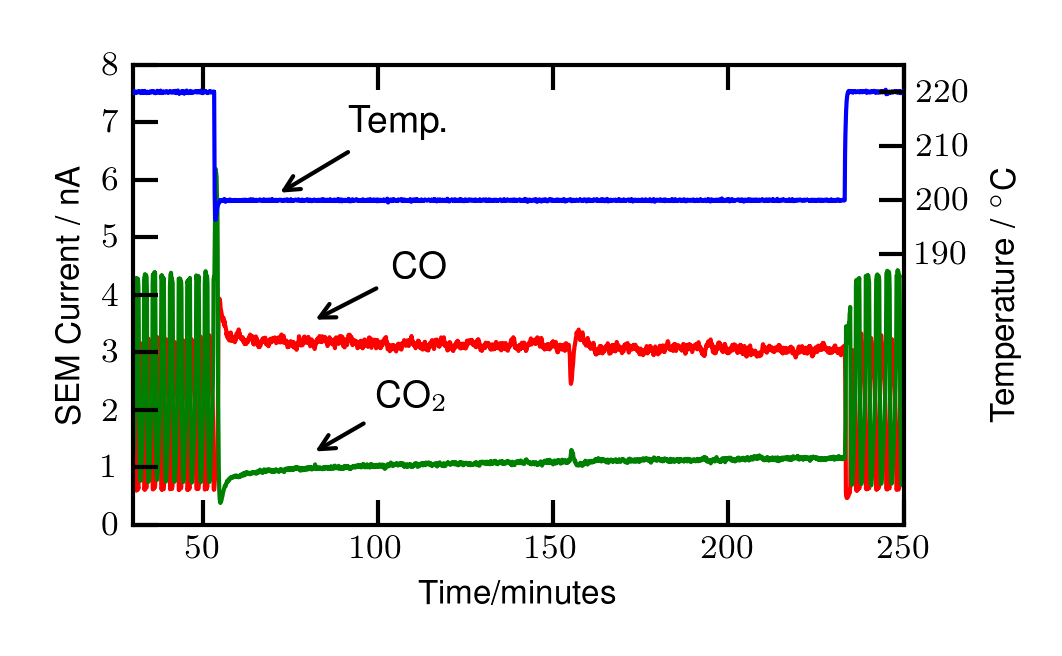
\includegraphics[width=12cm]{temperature_dependence_supplemental.png}
  \caption{Another example of the very pronounced temperature dependence.}
  \label{fgr:temperature_dependence_supplemental}
\end{figure}

\subsection{Duty cycle}
Even though the period of the oscillations increases with time the total
integrated conversion rate during a complete cycle is almost constant. In
\ref{fgr:duty_cycles_supplemental} the mean value of CO and
CO$_2$ is plotted for every oscillation in a four-day long experiment. It is
evident that the ratio between CO and CO$_2$ is almost constant. The
average activity of the sample is thus almost unchanged despite the development in
the oscillation frequency.

\begin{figure}
  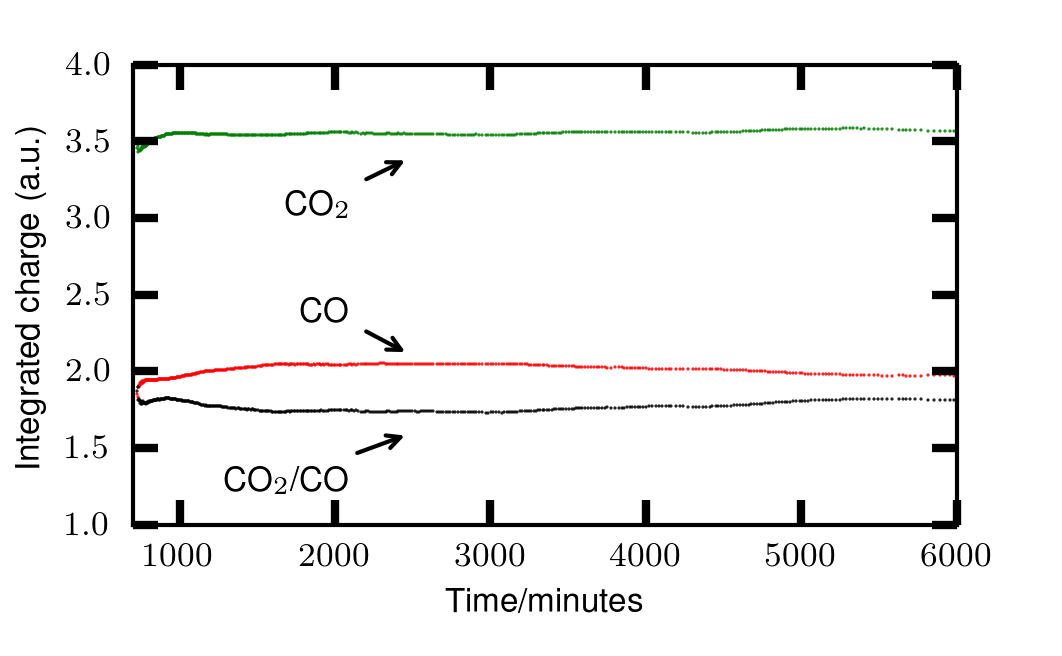
\includegraphics[width=12cm]{duty_cycles_long_measurement_supplemental.png}
  \caption{Running average of the CO and CO$_2$ concentrations and their ratio
  during a 4-day long experiment. The individual data-points is calculated as
  the integral of CO (red) or CO$_2$ (green) during the individual oscillation
  periods. The ratio between CO and CO$_2$ is drawn in black.}
  \label{fgr:duty_cycles_supplemental}
\end{figure}


\end{document}
